%%%%%%%%%%%%%%%%%%%%%%%%%%%%%%%%%%%%%%%%%
% Beamer Presentation
% LaTeX Template
% Version 1.0 (10/11/12)
%
% This template has been downloaded from:
% http://www.LaTeXTemplates.com
%
% License:
% CC BY-NC-SA 3.0 (http://creativecommons.org/licenses/by-nc-sa/3.0/)
%
%%%%%%%%%%%%%%%%%%%%%%%%%%%%%%%%%%%%%%%%%

%----------------------------------------------------------------------------------------
%	PACKAGES AND THEMES
%----------------------------------------------------------------------------------------

\documentclass{beamer}

\mode<presentation> {

% The Beamer class comes with a number of default slide themes
% which change the colors and layouts of slides. Below this is a list
% of all the themes, uncomment each in turn to see what they look like.

%\usetheme{default}
%\usetheme{AnnArbor}
%\usetheme{Antibes}
%\usetheme{Bergen}
%\usetheme{Berkeley}
%\usetheme{Berlin}
%\usetheme{Boadilla}
%\usetheme{CambridgeUS}
%\usetheme{Copenhagen}
%\usetheme{Darmstadt}
%\usetheme{Dresden}
%\usetheme{Frankfurt}
%\usetheme{Goettingen}
%\usetheme{Hannover}
%\usetheme{Ilmenau}
%\usetheme{JuanLesPins}
%\usetheme{Luebeck}
%\usetheme{Madrid}
%\usetheme{Malmoe}
%\usetheme{Marburg}
%\usetheme{Montpellier}
%\usetheme{PaloAlto}
%\usetheme{Pittsburgh}
%\usetheme{Rochester}
%\usetheme{Singapore}
%\usetheme{Szeged}
\usetheme{Warsaw}

% As well as themes, the Beamer class has a number of color themes
% for any slide theme. Uncomment each of these in turn to see how it
% changes the colors of your current slide theme.

%\usecolortheme{albatross}
\usecolortheme{beaver}
%\usecolortheme{beetle}
%\usecolortheme{crane}
%\usecolortheme{dolphin}
%\usecolortheme{dove}
%\usecolortheme{fly}
%\usecolortheme{lily}
%\usecolortheme{orchid}
%\usecolortheme{rose}
%\usecolortheme{seagull}
%\usecolortheme{seahorse}
%\usecolortheme{whale}
%\usecolortheme{wolverine}

%\setbeamertemplate{footline} % To remove the footer line in all slides uncomment this line
%\setbeamertemplate{footline}[page number] % To replace the footer line in all slides with a simple slide count uncomment this line

%\setbeamertemplate{navigation symbols}{} % To remove the navigation symbols from the bottom of all slides uncomment this line
}

\usepackage[utf8]{inputenc}
\usepackage{graphicx} % Allows including images
\usepackage{booktabs} % Allows the use of \toprule, \midrule and \bottomrule in tables
\setbeamertemplate{caption}[numbered]
\usepackage{amsmath,amsfonts,amsthm,amssymb,graphicx,mathtools,tikz,hyperref} \renewcommand\qedsymbol{$\blacksquare$}
\usetikzlibrary{positioning}

\usepackage{listings}


\newcommand{\N}{\mathbb{N}}
\newcommand{\Z}{\mathbb{Z}}
\newcommand{\Q}{\mathbb{Q}}
\newcommand{\CX}{\mathbb{C}}
\newcommand{\R}{\mathbb{R}}
\newcommand{\F}{\mathbb{F}}
\newcommand{\Oc}{\mathcal{O}}
\newcommand{\ita}[1]{\textit{#1}}
\newcommand{\com}[2]{#1\backslash#2}
\newcommand{\oneton}{\{1,2,3,...,n\}}
\newcommand\idea[1]{\begin{gather*}#1\end{gather*}}
\newcommand\ef{\ita{f} }
\newcommand\eff{\ita{f}}
\newcommand\proofs[1]{\begin{proof}#1\end{proof}}
\newcommand\inv[1]{#1^{-1}}
\newcommand\setb[1]{\{#1\}}
\newcommand\en{\ita{n }}
\newcommand{\vbrack}[1]{\langle #1\rangle}
\DeclareMathOperator{\ord}{ord}
\DeclareMathOperator{\Char}{char}

% \theoremstyle{plain}
% \newtheorem{theorem}{Teorema}
% \newtheorem{lemma}[theorem]{Lema}
% \newtheorem{proposition}[theorem]{Proposición}
% \newtheorem*{corollary}{Corolario}

\theoremstyle{plain} % just in case the style had changed
\newcommand{\thistheoremname}{}
\newtheorem*{genericthm}{\thistheoremname}
\newenvironment{namedtheorem}[1]
  {\renewcommand{\thistheoremname}{#1}%
   \begin{genericthm}}
  {\end{genericthm}}

\theoremstyle{definition}
% \newtheorem*{definition}{Definición}

\theoremstyle{remark}
\newtheorem*{remark}{Remark}
\newtheorem*{claim}{Claim}

%----------------------------------------------------------------------------------------
%	TITLE PAGE
%----------------------------------------------------------------------------------------

\title[Finding Maximal and Optimal Elliptic Curves]{Finding Maximal and Optimal Elliptic Curves} % The short title appears at the bottom of every slide, the full title is only on the title page

\author{Alec Zabel-Mena} % Your name
\institute[UPR-RP] % Your institution as it will appear on the bottom of every slide, may be shorthand to save space
{
Universidad de Puerto Rico, Recinto de Rio Piedras \\ % Your institution for the title page
}
\date{\today} % Date, can be changed to a custom date

\begin{document}

\begin{frame}
\titlepage % Print the title page as the first slide
\end{frame}


%----------------------------------------------------------------------------------------
%	PRESENTATION SLIDES
%----------------------------------------------------------------------------------------

\section{Preliminary Definitions}
\begin{frame}
\frametitle{Groups}

\begin{definition} A nonempty set $G$ with a binary operation $\cdot$ is called a \textbf{group} for for all  $a,b,c \in G$
    \begin{enumerate}
        \item $a\cdot{b} \in G$.
        \item  $a\cdot{(b\cdot{c})}=(a\cdot{b})\cdot{c}$.
        \item $ \exists e \in G$ such that $ \forall a \in G$, $a\cdot{e}=e\cdot{a}=a$
        \item $\forall a \in G$ $\exists a^{-1} \in G$ such that, $a\cdot{a^{-1}}=a^{-1}\cdot{a}=e$.
    \end{enumerate}
\end{definition}

\begin{definition}
    A group $G$ is \textbf{abelian}  (or \textbf{commutative}) if for $a,b \in G$, $a\cdot{b}=b\cdot{a}$.
\end{definition}

\end{frame}

\begin{frame}
\frametitle{Examples of Groups}
\begin{itemize}
    \item The group of integers $\Z$.
    \item The group of integers modulo $n$, $\Z/n\Z$.
    \item The group of units of $\Z/n\Z$, $U(\Z/n\Z)$.
\end{itemize}


\end{frame}

\begin{frame}
\frametitle{Fields}

\begin{definition} A nonempty subset $F$, together with binary operations $+$ and $\cdot$, is called a \textbf{field} if it satisfies the following:
    \begin{enumerate}
        \item $(F,+)$ is an abelian group.
        \item $(F,\cdot)$ is an abelian group.
        \item For $a,b,c \in F$, $a\cdot(b+c)=a\cdot{b}+a\cdot{c}$.
    \end{enumerate}

\end{definition}

\begin{definition}
    For a field $F$, the \textbf{characteristic} of $F$ is the smallest positive integer $p$ such that $pa=0$. We denote it by $\Char{F}=p$
\end{definition}


\end{frame}

\begin{frame}
\frametitle{Examples of Fields}
\begin{itemize}
    \item The field of real numbers $\R$.
    \item The field of rational numbers$\Q$.
    \item The field of complex numbers$\CX$.
    \item Finite fields, $\F_p$, where $\Char{\F_p}=p$.
\end{itemize}


\end{frame}

\section{Elliptic Curves}
\begin{frame}
\frametitle{Definition}

\begin{definition} 
    Let $K$ be a field, and let $f(x)=x^3+a_2x^2+a_4x+a_6 \in K[x]$ a cubic polynomial with no multiple roots. The \textbf{elliptic curve} is the polynomial
        \begin{equation}
            y^2+a_1xy+a_3y=f(x)
        \end{equation}
    together with a \textbf{point at infinity} $\Oc$.

\end{definition}

\end{frame}

\begin{frame}
\frametitle{Examples.}
\begin{figure}
    \centering
    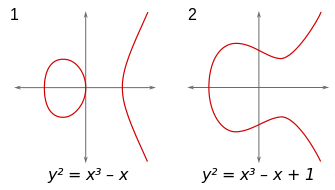
\includegraphics{Figures/ECClines-3.jpg}
    \caption{}
    \label{fig:my_label}
\end{figure}


\end{frame}

\begin{frame}
\frametitle{The Addition Law on Elliptic Curves}

Let $E(K)$ be an elliptic curve over a field $K$. We define the addition of points of $E(K)$ to be the binary operation $+$ such that $\forall P,Q,R \in E(K)$: 

\begin{itemize}
    \item If $P=\mathcal{O}$, Then $-P=\mathcal{O}$ and $P+Q=Q$.
    
    \item If $P=(x,y) \in E(K)$ then $-P=(x,-a_1x-a_3-y) \in E(K)$.
    
    \item If $P \neq Q$, take the line $l=\overline{PQ}$ to be the line that cuts $E(K)$ at $P$, $Q$, and another point $R$. Then $P+Q=-R$.
    
    \item If $P = Q$, take the line $l=\overline{PQ}$ tangent at $P$ cutting another point $R$. Then $P+Q=-R$.
\end{itemize}


\end{frame}

\begin{frame}
\frametitle{The addition law}

\begin{figure}
    \centering
    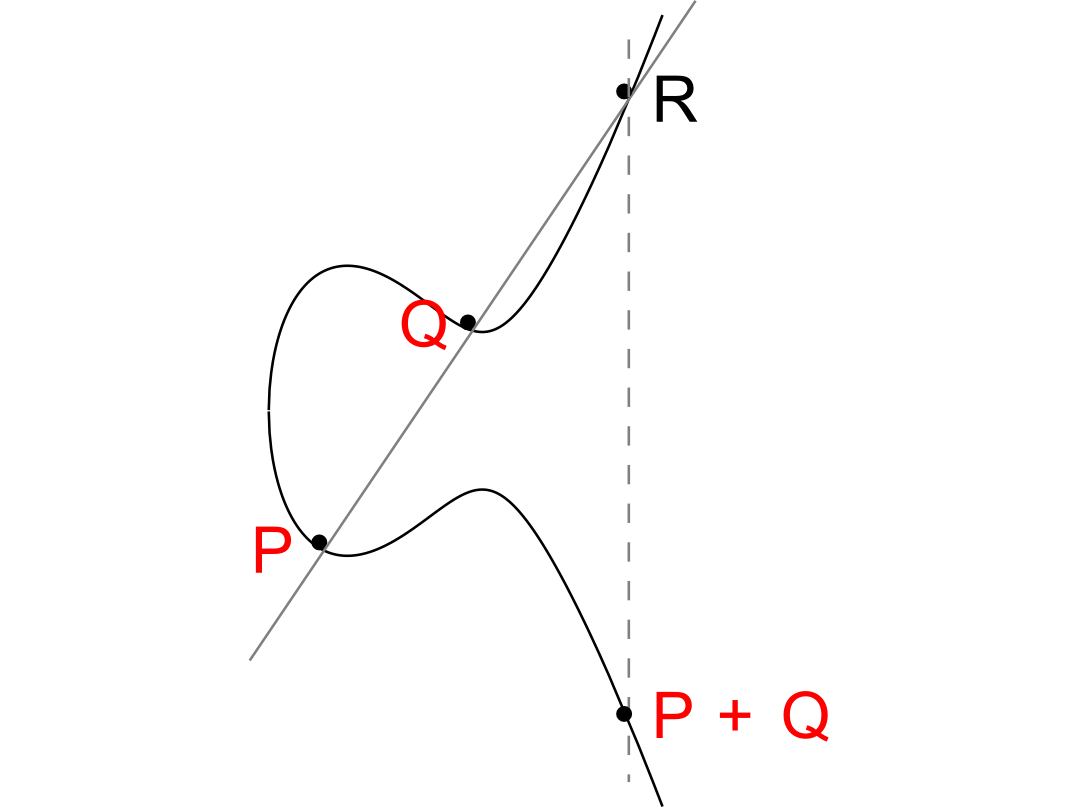
\includegraphics{Figures/EllipticCurveAddition}
    \caption{}
    \label{fig:my_label}
\end{figure}



\end{frame}


\section{Maximal and Optimal Curves}
\begin{frame}
\frametitle{The Zeta Function of an Elliptic Curve}
    \begin{itemize}
        \item Consider the Elliptic Curve $E$ defined over $\F_q$. Then $E$ is defined over any extension field $\F_{q^r}$ for $r \in \Z^+$
        
        \item We denote $N_r=|E(\F_{q^r})|$ to be the number of $\F_{q^r}$ \textbf{rational points} on $E$.
        
        \item $N_1=N=|E(\F_q)|$
    \end{itemize}


\end{frame}

\begin{frame}
\frametitle{The Zeta Function of an Elliptic Curve}
    
\begin{definition}
    We define the \textbf{Zeta function} of the elliptic curve $E$ over $\F_q$ to be the formal power series over $\Q[[T]]$ defined by:
    \begin{equation}
        Z(E/\F_q)=\exp{(\sum_{r} \frac{N_rT^r}{r})}
    \end{equation}
\end{definition}

\begin{itemize}
    \item The Weil conjectures give an explicit formula for the zeta fucntion of an elliptic curve
\end{itemize}


\end{frame}


\begin{frame}
\frametitle{The Zeta Function of an Elliptic Curve}
    
\begin{theorem}[The Weil Conjectures for an Elliptic Curve]
    Let $E$ be an elliptic curve over $\F_q$. The zeta function of $E$ is the rational function of $T$ of the form:
        \begin{equation}
            Z(E/\F_q,T)=\frac{1-aT+qT^2}{(1-T)(1-qT)}
        \end{equation}
\end{theorem}

\begin{itemize}
    \item Where $N_1=q+1-a$.
    
    \item We can also find $a=\alpha+\beta$ where $\alpha$ and $\beta$ is a complex conjugate pair such that $|\alpha|=|\beta|=\sqrt{q}$.
    
    \item By knowing $N_1$ and finding $\alpha$ and $\beta$ one can find the number of $\F_{q^r}$ rational points by taking: $N_r=q^r+1-\alpha^r-\beta^r$
\end{itemize}


\end{frame}

\begin{frame}
\frametitle{The Hasse Bound}
    
\begin{theorem}[Hasse's Theorem]
    Let $N$ be the number of $\F_q$ rational points on an elliptic curve $E(\F_q)$. Then:
    \begin{equation}
        |N-(q+1)| \leq 2\sqrt{q}
    \end{equation}
\end{theorem}

\begin{itemize}
    \item Hasse's theorem provides a good bound for testing whether certain elliptic curves are optimal optimal, or maximal.
    
    \item We find such curves.
\end{itemize}

\end{frame}

\begin{frame}
\frametitle{The Hasse Bound}
    
\begin{verbatim}

q = 2
r = 2 

for a6 in range(q):
    for a4 in range(q):
        for a3 in range(q):
            for a2 in range(q):
                for a1 in range(q):
                    b2=a1^2+4*a2; b4=a1*a3+2*a4; b6=a3^2+4*a6; b8=a1^2*a6-a1*a3*a4+a2*a3^2+4*a2*a6-a4^2
   
\end{verbatim}

\end{frame}




%------------------------------------------------


\begin{frame}{References}


 
\end{frame}



%----------------------------------------------------------------------------------------

\end{document}
